\documentclass[12pt, titlepage]{report}
\usepackage{consumer_resource_final}
\graphicspath{{./figures/}}

\begin{document}

We want to be able to build feasible models numerically, \ie we would like to generate a set of constant numbers $\{
l_\nu, m_\nu, R^*_\nu, S^*_j, \gamma_{j\nu}, \alpha_{\nu j}, \sigma_{j\nu}\}$ such that the equilibria equations Eqs.\eqref{eq : equilibrium resources and species} are fulfilled.


\subsection{Algorithmic procedure}\label{sec : algorithmic procedure}
We hereby detail the procedure used to numerically build feasible systems. It goes like this:
\begin{enumerate}
  \item We first draw randomly each $R^*_\nu$
  and $S^*_i$ from a uniform distribution of mean equal to the corresponding metaparameter, \ie :
  \begin{equation}
     R^*_\nu = \mathcal{R} \ \forall \nu=1, \dots, N_R\text{ and }  S^*_i = \mathcal{S} \ \forall i=1, \dots, N_S,
  \end{equation}
  where $\mathcal{R}$ and $\mathcal{S}$ are random variables coming from a distribution of mean equal to the corresponding metaparameter and relative standard deviation\footnote{By relative standard deviation, we mean the standard deviation measured in units of the average value.} $\epsilon$. In our simulations, we chose uniform distributions :
  \begin{equation}
  \mathcal{R} \sim \text{Unif}(R_0, \epsilon) \text{ and } \mathcal{S} \sim \text{Unif}(S_0, \epsilon).
  \end{equation}
  \item The efficiency matrix $\sigma_{i\nu}$ is then drawn similarly, from a distribution with average $\sigma_0$. In order to simplify the problem\footnote{Indeed, a non uniform $\sigma_0$ introduces instability in the system}, we will take a zero-variance à la \citeauthor{butler_stability_2018} in \cite{butler_stability_2018}, \ie all species consume resources at the same global efficiency :
  \begin{equation}
    \sigma_{i\nu} = \sigma_0.
  \end{equation}
  \item We build the consumption matrix $\gamma_{i\nu}$. Its adjacency matrix $G$ is loaded through a user-provided file.
  %$G$ is a binary matrix given by the user (in the \code{configuration.in} file) and is defined as the adjacency matrix of the consumption network (\ie it tells which species eats which resource). We then build $\gamma$ with the same network structure as $F$ (\ie both matrices have the same zero elements).
  While $G$ gives the structure of $\gamma$, \ie if a given $\gamma_{i\nu}$ is zero or not, the actual values of $\gamma_{i\nu}$ need then to be determined. They are drawn from a uniform distribution of mean $\gamma_0$ and relative standard deviation $\epsilon$:
  \begin{equation}
    \gamma_{i\nu} = \text{Unif}(\gamma_0, \epsilon) G_{i\nu}.
  \end{equation}
  \item We draw the resources external feeding rates, similarly to the other parameters :
  \begin{equation}
  l_\mu = \text{Unif}(l_0, \epsilon) \ \forall \mu=1, \dots, N_R.
  \end{equation}
  \item The last free parameter is the syntrophy matrix $\alpha_{\nu i}$, the $d_i$ and $l_\mu$ are determined through the equations of evolution at equilibrium. This is the tricky part of the algorithm because $\alpha$ has to follow three constraints, namely energy conservation/dissipation Eq.\eqref{eq : dissipation constraint} and positiveness of $d_i$ and $l_\mu$ [\textbf{insert reference to equation}]. The general strategy is to choose the metaparameters in a way that these constraints should \textit{almost always} be satisfied, \ie we pick metaparameters that follow the feasibility constraint Eq.\eqref{eq : overall feasibility constraint metaparameters}. The adjacency matrix $A$ of $\alpha$ needs then to be specified. At the moment, it can be chosen in three different ways : fully connected, or in a way that no resource eaten by a given species can be released by that same species (\ie $G_{i\mu}>0 \iff A_{\mu i}=0$) or by a user provided matrix. After the adjacency matrix is loaded, we can build $\alpha$ from a uniform distribution of mean $\alpha_0$ and relative standard deviation $\epsilon$:
  \begin{equation}
    \alpha_{\nu i} = \text{Unif}(\alpha_0, \epsilon) A_{\nu i} .
  \end{equation}
  %\item We build $\tau_{\nu i}$. It usually is equal to $\alpha_{\nu i}$ or 0.
  \item With all of these parameters drawn, we can solve Eq.\eqref{eq : equilibrium species} for the species death rate $d_i$.
  \item We solve Eq.\eqref{eq : equilibrium resources} for $m_\nu$. All the parameters of the model are now fully determined.
  \item We check if the constraints Eq.\textbf{(insert reference)} on the parameters are fulfilled. If they are not, we go back to step 1. Otherwise, we can exist the algorithm, a feasible system has been built.
\end{enumerate}

\subsection{Basic concepts}
Since its very inception \cite{may_will_1972}, the study of ecological interactions has been and still is tightly close to the one of random matrices \cite{allesina_stability_2012, allesina_predicting_2015, barbier_cavity_2017}. Usually, the procedure is assuming we are at a feasible equilibrium point, where some matrix of the model (\eg the species-interaction matrix or the jacobian) is approximated as random, and then study the dynamical stability of said feasible point.

This framework is not satisfying for the study we would like to conduct, because the question ``does a given set of random parameters lead to a feasible system?'' is not trivial at all. Indeed for our model to make sense, we impose two conditions on any system deemed as feasible : the model parameters must be ``biological'' and biomass must be conserved.

Asking for the model parameters to be biological simply means we want them to have the intended biological interpretation. This means \eg that any syntrophic interaction has to be non-negative $\alpha_{\mu i} \geq 0 $ otherwise it cannot be interpreted as a syntrophic interaction anymore. More generally this is equivalent to requiring that all the model parameters are non-negative:
\begin{equation}
 p \geq 0 \ \forall p \in \mathcal{P}.
\end{equation}
In our study, this equation will be slightly restricted since we are looking for positive-valued equilibria, so we require
$R^*_\mu, S^*_i > 0$ specifically for these two parameters. Also, we require also a non-zero efficiency\footnote{It wouldn't make sense to say that species $i$ eats resource $\mu$ with efficiency $0$, since this is equivalent to species $i$ not eating resource $\mu$, and this is already encoded in the network structure.}. Finally every resource feeding rate should be non-zero in order to avoid resource depletion and every resource and consumer must eventually die out in the absence of interaction. In the end this means we require:
\begin{equation}
R^*_\mu, S^*_i, \sigma_{i\mu}, l_\mu, d_i, m_\mu, \sigma_{i\mu} > 0 \text { and } \gamma_{i\mu}, \alpha_{\mu i} \geq 0. \label{eq : feasibility positive parameters}
\end{equation}
Remember that not all the parameters of our models are free : there are $3 N_R +2 N_S + 4 N_R N_S $ parameters constrained by $N_R + N_S $ equations. So if we set $2 N_R + N_S + 4 N_R N_S$ parameters, the remaining $N_R + N_S$ are not free but set by the equilibrium equations \textbf{Insert ref equation}. Traditionally, we would solve for $R^*$ and $S^*$ and choose the rest of the parameters, but for reasons explained in \textbf{insert ref}, we will solve for the consumers death rates $d_i$ and the resources diffusion rate $m_\mu$. This means that if we \textit{choose} non-negative $\gamma, \alpha, \sigma, \tau, l, R^*$ and $S^*$, Eq.\eqref{eq : feasibility positive parameters} is equivalent to :
\begin{subequations}\label{eq : feasibility positive d and m}
\begin{empheq}[left=\empheqlbrace]{align}
d_i &= \sum_\nu \left( \sigma_{i\nu} \gamma_{i\nu} R_\nu - \alpha_{\nu i} \right) > 0 \ \forall i=1, \dots, N_S \\
m_\mu &= \frac{l_\mu - \sum_j \left(\gamma_{j\mu}R_\mu-\alpha_{\mu j}\right)S_j}{R_\mu} > 0 \ \forall \mu = 1, \dots, N_R
\end{empheq}
\end{subequations}

In addition to Eqs.\eqref{eq : feasibility positive d and m}, we want any feasible system to conserve biomass \important{at equilibrium}\footnote{This weak condition should hold only at equilibrium : we allow transition periods where biomass may not be conserved.}. This means no species should be able to produce more biomass than it physically can. More specifically, a consumer $i$ attains, from consuming resources, a total biomass of $\sum_\nu \gamma_{i\nu}R^*_\nu S^*_i$.
From this available biomass, only a part $\sum_\nu \sigma_{i\nu}\gamma_{i\nu}R^*_\nu S^*_i$ is devoted to growth. From the remaining $\sum_\nu (1-\sigma_{i\nu})\gamma_{i\nu}R^*_\nu S^*_i$, a part $\sum_\nu \alpha_{\nu i} S^*_i$ is given back to the resources as a syntrophic interaction. We simply impose that the syntrophic interaction is smaller than or equal to the available remaining biomass :
\begin{equation}\label{eq : feasability biomass conservation}
 \sum_\nu (1-\sigma_{i\nu})\gamma_{i\nu}R^*_\nu  \geq \sum_\nu \alpha_{\nu i} \ \forall i=1, \dots, N_S.
\end{equation}
From now on, we will say that a parameter set $p$ is \define{feasible} if it satisfies Eqs.\eqref{eq : feasibility positive d and m} and \eqref{eq : feasability biomass conservation}.
This is completely deterministic, in the sense that for a given parameters set $p \in \mathcal{P}$ one can without a doubt say whether it is feasible or not.
We can hence define the \define{parameters set feasibility function} $\mathfrak{F} : P \rightarrow \{ 0, 1 \}$, which takes a parameter set as an input and tells you whether this parameter set is feasible or not:
\begin{equation}
\mathfrak{F}(p)=
\begin{cases}
1 \text{ if }p \text{ is feasible,} \\
0 \text{ else.}
\end{cases}
\end{equation}
However as explained above we will usually not work with a parameter set $p \in \mathcal{P}$ directly -- because there are too many variables to keep track of -- but with a metaparameter set $m \in \mathcal{M}$ and a binary consumption matrix $G \in \mathcal{B}_{N_R \times N_S}$ instead. We can similarly define a
\define{metaparameters set feasibility function} $\mathcal{F} : \mathcal{M} \rightarrow [0, 1] \times \mathcal{B}_{N_R \times N_S}$ which is the probability that a given set of metaparameters $m \in \mathcal{M}$ coupled with binary matrices $B=(G, A)$ gives rise -- through the algorithmic procedure $\mathcal{A}$ -- to a feasible parameter set :
\begin{equation}\boxed{
\mathcal{F}(m, B)=\text{Probability}\left\{\mathfrak{F}\left(\mathcal{A}(m, B)\right)=1\right\}
}
\end{equation}
We will in general work with $\mathcal{F}$ rather than $\mathfrak{F}$ because it is easier to handle metaparameters. In practice $\mathcal{F}(m, B)$ is estimated numerically by generating $N$ parameters sets from $(m,B)$ and calculating the number of feasible ones :
\begin{equation}
\mathcal{F}(m, B) = \lim_{N\rightarrow \infty} \sum_{i=1}^N \frac{\mathfrak{F}(\mathcal{A}(m,B))}{N} \approx \sum_{i=1}^N \frac{\mathfrak{F}(\mathcal{A}(m,B))}{N} \text{ for } N \gg 1.
\end{equation}

\subsection{The feasibility volume}
The algorithmic procedure above explains how feasible systems can be built. However, it implies that we first found a combination of metaparameters that will most of the time lead to the realisation of feasible systems when they are taken as an input of the algorithm.

Overall we have six metaparameters that we can play with : $\gamma_0$, $\alpha_0$, $l_0$, $\sigma_0$, $S_0$ and $R_0$. However, following the analysis of \cite{barbier_cavity_2017}, we notice that our system \eqref{eq : differential eq for resources and species} is arbitrary on some level. Indeed we have a ``scale freedom'', that means we decide in which set of units we work. There are two physical quantities at stake here : biomass and time, and we may choose, however we want it, a specific set of units describing both of them.

We will measure biomass in units of the average resource abundance at equilibrium\footnote{Note that this is not a completely innocent choice. Indeed we will see later that the matrix $\alpha_{\nu i}-\gamma_{i \nu} R^*_\nu$ is a crucial quantity here. Setting $\av{R^*}=1$ allows us to simply study the impact of $\gamma$ against $\alpha$ instead of the more complicated $\gamma R^*$ versus $\alpha$.}, that means :
\begin{equation}
 \av{R_\mu} = R_0 = 1.
\end{equation}
Similarly, we will measure time such that the average external resource uptake rate is one, that is :
\begin{equation}
\av{l_\mu} = l_0 = 1.
\end{equation}
After this manipulation, our number of metaparameters is reduced from six to four : only $\gamma_0$, $S_0$, $\alpha_0$ and $\sigma_0$ remain.

For the sake of simplicity, we will keep the same $\sigma_0$ throughout our whole study. We take a value close to the efficiency of real microbial systems [\textbf{insert ref}], that is $\sigma_0 =0.3$.

Overall, we need to choose the last three remaining metaparameters: $\alpha_0$, $\gamma_0$ and $S_0$. What Eq.\eqref{eq : overall feasibility constraint metaparameters} tells us is that as soon if we choose $\gamma_0$ and $S_0$, we will get a feasibility range for $\alpha_0$.
We will then choose $\gamma_0$ and $S_0$ such that they lead to feasible systems for every consumption matrix considered here \textbf{when there is no syntrophy}, \ie $\alpha_0=0$. We will then study the impact of varying $\alpha_0$ at those values of $\gamma_0$ and $S_0$.

Formally, we can define for a consumption adjacency matrix $G$ the volume $\mathcal{V}^G_x$ of the metaparameters space that will lead to at least a ratio $x$ of feasible systems \ie :
\begin{equation}
\mathcal{V}^G_x \defined \left\{m \in \mathcal{M} : \mathcal{F}(m, G)\geq x \right\}.
\end{equation}
It is clear that $\mathcal{V}^G_0 = \mathcal{M}$ $\forall G$ and $\mathcal{V}^G_{x} \leq \mathcal{V}^G_{y}$ $\forall x > y, G$ . We can similarly define for a set $S = \left\{ G_1, G_2, \dots, G_N\right\}$ of $N$ matrices their \textit{common feasibility} volume $\mathcal{V}^S_x$, which is the region of the metaparameters space where feasibility is at least $x$ for every matrix in the set:
\begin{equation}
\mathcal{V}^S_x = \intersection{G \in S} \mathcal{V}^G_x.
\end{equation}
We also define for a matrix set $S$, its critical feasibility $x^*(S)$, which is the largest feasibility we can get while still having a non-zero common volume :
\begin{equation}
x^*(S) \defined \max_{x \in \left[0,1\right]}\left\{ x : \mathcal{V}^S_x > 0 \right\}.
\end{equation}
For actual computations, we will choose a matrix set $S_M$, stick to it during the whole thesis, and work in its critical feasibility volume $\mathcal{V}^*$, defined as :
\begin{equation}\boxed{
\mathcal{V}^* \defined \mathcal{V}^{S_M}_{x^*(S_M)}.
}
\end{equation}


\begin{figure}
\centering
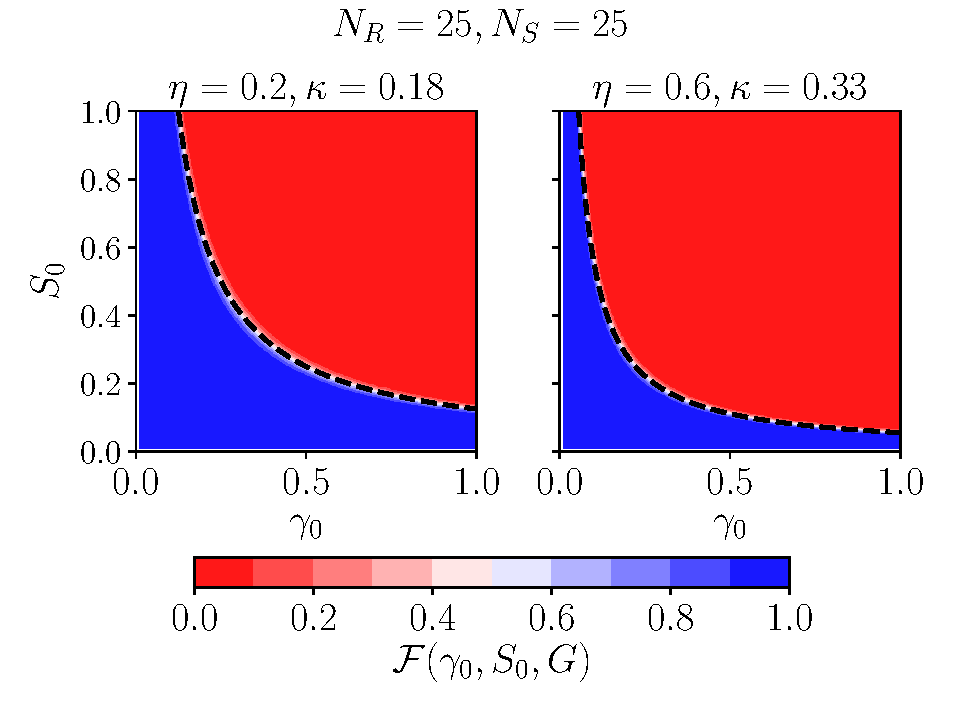
\includegraphics{Results/typical_feasibility_volume}
\caption{Plot of the feasability area. The color curve indicicates the feasibility function $\mathcal{F}$ for the matrix of our set with connectance $0.18$ and nestedness $0.15$ . We observe a steep descent from a totally feasible to totally unfeasible regime. A fit of the points $\mathcal{F}(\gamma_0, S_0) \approx 0.5 $ yields $S_0 = 0.17310809 \gamma_0 -0.0029606$
(with a relative error of $10^{-6}$). The theoretical prediction is $S_0 = 0.2 \gamma_0$. The full line indicates the theoretical critical feasibility volume, and the dashed area the measured one. Although not perfect it matches quite well. A fit yields $S_0 = 0.04261718 \gamma_0 -0.00456834$ with a relative error of the order of $10^{-6}$. Theoretical predicts $S_0=0.0526316 \gamma_0$}
\end{figure}


\end{document}
